\documentclass{article}
%\usepackage{enumitem}
\usepackage{listings}
\usepackage{amsfonts}
\usepackage{latexsym}
\usepackage{fullpage}
\usepackage{graphicx}
%\usepackage{paralist}
\usepackage{tikz-timing}
\usepackage{tabto}
\usepackage[utf8]{inputenc}
\usepackage[T1]{fontenc}
\usepackage{filecontents}
\usepackage[backend=biber,style=ieee]{biblatex}
\usepackage{caption}
\usepackage{subcaption}

\lstset{language=C}

\graphicspath{{images/}}

% Default margins are too wide all the way around. I reset them here
\setlength{\topmargin}{-.5in}
\setlength{\textheight}{9in}
\setlength{\oddsidemargin}{.125in}
\setlength{\textwidth}{6.25in}

% Defining references here

\begin{filecontents}{\jobname.bib}
@article{singh2014,
author = {Dhananjay, Singh and Gaurav, Tripathi},
year = {2014},
month = {03},
pages = {},
title = {A Survey of Internet-of-Things: Future Vision, Architecture, Challenges and Services},
journaltitle = {2014 IEEE World Forum on Internet of Things, WF-IoT 2014}
}
@online{arduinoblog,
author = {Arduino},
title = {Arduino Blog},
year = {2017},
url = {https://blog.arduino.cc},
OPTnote = {Acessado em 24 de Abril de 2017}
}
@article{santanna2012,
author = {Francisco Sant’Anna and
Noemi de La Rocque Rodriguez and
Roberto Ierusalimschy},
title = {CÉU: Embedded, Safe, and
Reactive},
journaltitle = {Monografias em Ciência da Computação},
year = {2012},
volume = {9},
issn = {0103-9741}
}
@online{githubceuarduino,
author = {Francisco Sant'Anna},
title = {GitHub Céu-Arduino},
year = {2017},
url = {https://github.com/fsantanna/ceu-arduino},
note = {Acessado em 24 de Abril de 2017}
}
@article{wortmann2015,
author = {Felix Wortmann and Kristina Flütcher},
year = {2015},
pages = {221-224},
title = {Internet of Things - Technology and Value Added},
journaltitle = {Business \& Information Systems Engineering},
volume = {57},
issue = {3}
}
@periodical{chui2010,
editor = {Michael Chui and Markus Löffer and Roger Roberts},
title = {The Internet of Things},
year = {2010},
series = {McKinsey Quarterly},
month = {Março},
url = {https://www.mckinsey.com/industries/high-tech/our-insights/the-internet-of-things}
}
@ARTICLE{edwards1997, 
author={S. Edwards and L. Lavagno and E. A. Lee and A. Sangiovanni-Vincentelli}, 
journal={Proceedings of the IEEE}, 
title={Design of embedded systems: formal models, validation, and synthesis}, 
year={1997}, 
volume={85}, 
number={3}, 
pages={366-390}, 
keywords={application specific integrated circuits;computer architecture;formal specification;formal verification;logic design;real-time systems;systems analysis;ASIC;application-specific integrated circuits;concurrent design process;embedded software;embedded systems design;formal models;formal validation;heterogeneous systems;reactive real-time system design;specification;Application software;Application specific integrated circuits;Computer architecture;Consumer electronics;Embedded computing;Embedded system;Hardware;Microcontrollers;Real time systems;Safety}, 
doi={10.1109/5.558710}, 
ISSN={0018-9219}, 
month={Mar},}
@online{githubceu,
author = {Francisco Sant'Anna},
title = {GitHub Céu},
year = {2017},
url = {https://github.com/fsantanna/ceu},
note = {Acessado em 24 de Abril de 2017}
}
@manual{atmegadatasheet,
author = {AtMel},
title = {AtMel ATmega328/P DATASHEET},
year = {2016},
organization = {ATMel},
}

\end{filecontents}

\addbibresource{\jobname.bib}

% End defining references

\begin{document}

\begin{titlepage}

\newcommand{\HRule}{\rule{\linewidth}{0.5mm}} % Defines a new command for the horizontal lines, change thickness here

\center % Center everything on the page
 
%----------------------------------------------------------------------------------------
%	HEADING SECTIONS
%----------------------------------------------------------------------------------------

\textsc{\LARGE Pontifícia Universidade Católica do Rio de Janeiro}\\[1.5cm] % Name of your university/college
\textsc{\Large Projeto Final de Graduação de Engenharia da Computação}\\[0.5cm] % Minor heading such as course title

\textsc{\large Departamento de Informática - DI \\ Centro Técnico Científico - CTC \\ Curso de Engenharia da Computação}\\[0.5cm] % Major heading such as course name


%----------------------------------------------------------------------------------------
%	TITLE SECTION
%----------------------------------------------------------------------------------------

\HRule \\[0.4cm]
{ \huge \bfseries Aplicação em Sistemas Distribuídos
utilizando biblioteca e driver próprios,
baseados em interrupções desenvolvido
em Céu para o microcontrolador Arduino}\\[0.4cm] % Title of your document
\HRule \\[1.5cm]
 
%----------------------------------------------------------------------------------------
%	AUTHOR SECTION
%----------------------------------------------------------------------------------------

\begin{minipage}{0.4\textwidth}
\begin{flushleft} \large
\emph{Aluno:}\\
Guilherme \textsc{Simas} % Your name
\end{flushleft}
\end{minipage}
~
\begin{minipage}{0.4\textwidth}
\begin{flushright} \large
\emph{Orientador:} \\
Ana \textsc{Lúcia de Moura} % Supervisor's Name
\end{flushright}
\end{minipage}\\[4cm]

% If you don't want a supervisor, uncomment the two lines below and remove the section above
%\Large \emph{Author:}\\
%John \textsc{Smith}\\[3cm] % Your name

%----------------------------------------------------------------------------------------
%	DATE SECTION
%----------------------------------------------------------------------------------------

{\large \today}\\[3cm] % Date, change the \today to a set date if you want to be precise

%----------------------------------------------------------------------------------------
%	LOGO SECTION
%----------------------------------------------------------------------------------------

%\includegraphics{Logo}\\[1cm] % Include a department/university logo - this will require the graphicx package
 
%----------------------------------------------------------------------------------------

\vfill % Fill the rest of the page with whitespace

\end{titlepage}

\newpage % Dedicatória

\begin{flushright}

\vspace*{\fill}

\textit{\LARGE Agradecimentos estarão descritos nesse bloco de texto. Caso o bloco de texto seja grande demais espera-se que ele pule linhas e continue se guiando pela margem direita}

\vspace*{\fill}

\end{flushright}

\newpage

\tableofcontents{}

\newpage

\section{Introdução}	


\tab Atualmente existe uma grande variedade de estudos e soluções no âmbito da Internet das Coisas
promovidos por empresas de tecnologia da informação, mostrando que o conceito pode ser
implementado e, embora não tenha uma presença evidente no dia-a-dia, está em constante
desenvolvimento e em processo de adequação. Existem várias definições do termo “Internet das
Coisas”, porém a grande maioria delas compartilha a opinião de que a conexão e troca de dados
entre elementos é parte vital do conceito. Por esse motivo, a área de Sistemas Distribuídos possui um
papel importantíssimo nesse desenvolvimento, já que toda aplicação deve ser capaz de trocar
mensagens e informação segura e corretamente de forma a se sincronizar, e de forma escalável. \cite{singh2014}
Outro ponto sobre a escalabilidade de aplicações em Internet das Coisas é a necessidade de unidades
computacionais de custo baixo e consumo eficiente de energia. Por esse motivo microcontroladores
são outra parte vital do desenvolvimento de soluções, apresentando, entre outras vantagens, uma
facilidade na programação devido a bibliotecas e drivers já implementados e disponibilizados.
Microcontroladores são capazes de processamento de dados por possuírem processadores e de
serem facilmente integrados com sensores e atuadores, possuindo hardware especializado para
interfacear com esses componentes.
\par Muitas APIs (conjuntos de rotinas, protocolos e ferramentas para desenvolvimento de software para
uma plataforma) fornecidas por microcontroladores incluem rotinas que causam um bloqueio na
aplicação, ou seja, enquanto está realizando a chamada correspondente àquela funcionalidade, o
software entra em um estado onde realiza tarefas virtualmente inúteis até que o hardware conclua sua
parte. Esse comportamento é indesejável visto que a aplicação desperdiça tempo aguardando o
hardware enquanto poderia estar realizando outras tarefas como, por exemplo, um processamento de
dados recebidos por uma mensagem, ou a troca de mensagens em si. Essa ineficiência marca um
desperdício de tempo e consumo de energia.
\par O bloqueio de aplicações é um desafio enfrentado frequentemente em aplicações que envolvem
sistemas nos quais o tempo de processamento ou reação a estímulos externos é pertinente ao
funcionamento da aplicação. O paradigma de programação orientada a eventos é muitas vezes
utilizado como abordagem nessas situações. Em uma aplicação orientada a eventos, o sistema segue
seu fluxo normal até a chegada de um “evento”, como a chegada de uma mensagem, ou a conclusão
de um trabalho por parte do hardware. A chegada de tal evento emite uma interrupção no sistema, que
irá executar uma rotina de tratamento desse evento, e após terminado, irá retomar seu fluxo normal
de execução, a partir de onde estava no momento da interrupção. Esse paradigma busca evitar que
quaisquer estímulos sejam ignorados involuntariamente pela aplicação ou que ciclos computacionais
sejam desperdiçados. Essa estruturação introduz uma espécie de paralelismo e imprevisibilidade no
fluxo de execução da aplicação, algo que linguagens comumente utilizadas para programação de
sistemas embarcados, como C, não fazem um bom papel de representar, por serem historicamente
procedurais (espera-se que o fluxo de execução siga naturalmente a ordem de leitura do código, a
linha de baixo imediatamente seguindo a execução da linha de cima).
\par Dentre um número enorme de microcontroladores, a plataforma Arduino possui uma comunidade de desenvolvedores e recebe muita atenção, além de ser open-source. Contribuições na forma de
exemplos de aplicações e desenvolvimento de drivers e bibliotecas são frequentes e são o que tornam
a comunidade tão bem-sucedida. Por último, a plataforma é de fácil acesso e muitas vezes utilizada
como parâmetro, devido à sua popularidade. \cite{arduinoblog}
\par Céu é uma linguagem de programação estruturada síncrona reativa, onde a orientação a eventos é
inerente à programação, assim como o paralelismo entre seções de código que surgem com esse
paradigma, como mencionado anteriormente. A linguagem, portanto, faz um ótimo papel de
implementar a orientação a eventos. Outro benefício de Céu é o fato de que a ordem de execução de
trechos de programa que estão descritos para rodar em paralelo é previsível dado a chegada de um
determinado evento. \cite{santanna2012} Devido às vantagens dessas características para a programação de
componentes de sistemas embarcados, foi desenvolvido um kit de desenvolvimento em Céu para
uma família de microcontroladores, Arduino, chamada Céu-Arduino.
\par Céu-Arduino permite a programação de microcontroladores Arduino utilizando a linguagem Céu, o
que facilita a programação orientada a eventos. Céu-Arduino, porém, não reimplementa os drivers e
bibliotecas desenvolvidos para Arduino em outras linguagens, e, portanto, não pode impedir o
bloqueio da aplicação que é consequência da chamada de funções bloqueantes pré-desenvolvidas. A
re-implementação desses módulos eliminaria mais uma possibilidade de bloqueio de uma aplicação
que as utilize. \cite{githubceuarduino}
\par Esse trabalho propõe reimplementar drivers e bibliotecas de Arduino, que atualmente causam
bloqueio da aplicação, de forma a que esse bloqueio não ocorra mais. A abordagem utilizada nesse
desenvolvimento será do uso de interrupções suportadas por hardware especializado com orientação a
eventos e, por esse motivo, a linguagem escolhida para esse desenvolvimento será Céu-Arduino. Os
resultados desse desenvolvimento serão publicados na página open-source de desenvolvimento do
kit, para que futuros desenvolvedores possam fazer uso de tais módulos em suas próprias aplicações
e objetivos.
\par Por fim, será desenvolvida uma aplicação em Sistemas Distribuídos para exemplificar a pertinência
dos módulos desenvolvidos. A aplicação consistirá em uma rede de sensores e atuadores na
plataforma Arduino, utilizando troca de mensagens. Alguns exemplos de aplicações que satisfazem
os requisitos e objetivos são: Um sistema de iluminação inteligente; um sistema de irrigação
monitorada; um controlador de tráfego. Esse trabalho tem como meta servir como uma contribuição
para a comunidade desenvolvedora de sistemas embarcados e de aplicações de IoT, assim como
desenvolvedores da plataforma Arduino. \cite{wortmann2015} \cite{chui2010} \cite{edwards1997} \cite{githubceu} \cite{atmegadatasheet}

\section{Estado da Arte}

\tab Bloqueios em chamadas de drivers de microcontroladores são comumente causados por
implementações que usam polling para checar se a operação foi concluída. Polling é caracterizado
quando o software constantemente checa um estado, aguardando uma mudança, para só então
prosseguir. Funcionalidades de hardware especializado em microcontroladores costumam sinalizar sua
conclusão mudando o estado de um registrador, caracterizando uma flag. Implementações não-
bloqueantes de chamadas de drivers podem envolver fazer com que a mudança de estado da flag cause
uma interrupção, de modo que o software não precisa ficar no estado de polling e possa usar o tempo
para realizar outras operações na aplicação, só retornando à chamada do driver quando este concluiu
sua tarefa. Caso não haja nenhuma tarefa a ser realizada, o microcontrolador pode entrar em um
modo de baixo consumo de energia, portanto sempre há ganhos por utilizar a abordagem não-
bloqueante.

\begin{figure}[hbp]
\centering
\begin{subfigure}[b]{.5\textwidth}
  \centering
  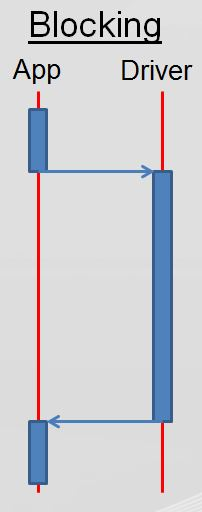
\includegraphics[width=.4\linewidth]{BlockingSequence}
  \caption{Comportamento blocante}
  \label{fig:sub1}
\end{subfigure}%
\begin{subfigure}[b]{.5\textwidth}
  \centering
  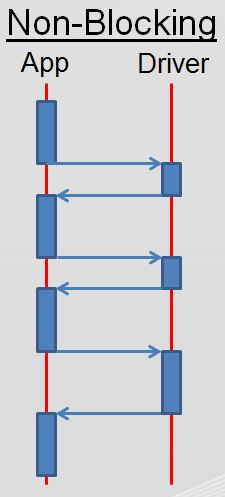
\includegraphics[width=.4\linewidth]{NonBlockingSequence}
  \caption{Comportamento não-blocante}
  \label{fig:sub2}
\end{subfigure}
\caption{Comparação entre comportamento blocante e não-blocante}
\label{fig:test}
\end{figure}

\par Kits de desenvolvimento para microcontroladores que ajudam a abstrair a implementação do
hardware do programador são sempre benéficos por tornarem o processo de desenvolvimento de
aplicações para aquele módulo mais simples e acessível. Microcontroladores Arduino são
normalmente programados em um ambiente de linguagem C, uma linguagem procedural, e os drivers
e bibliotecas disponibilizados pela própria Arduino apresentam atualmente funções e módulos que
causam o bloqueio da aplicação por utilizarem a técnica de polling. Embora existam reimplementações
por parte da comunidade de alguns desses módulos de forma a eliminar o bloqueio, Céu-Arduino
ainda não possui bibliotecas implementadas em Céu que resolvam o problema.
\par O kit de desenvolvimento Céu-Arduino apresenta uma abordagem única para o desenvolvimento
orientado a eventos e suporte a interrupções, e se encontra atualmente em um estado inicial. O
projeto está em uma versão 0.20 e conta com exemplos básicos de aplicações em Arduino queutilizam a linguagem Céu. Apesar de não possuir somente poucas bibliotecas e drivers desenvolvidos
em Céu, a linguagem é de fácil integração com C, sendo possível utilizar os módulos desenvolvidos
atualmente para Arduino. \cite{githubceuarduino}

\section{Results}
\tab Progress on each item in the previous section's list will now be presented below.
\subsection{Study current implementation of modules in Arduino which freeze the application}
\tab The Arduino programming model us structured, serial code. Fuctionalities are associated to function calls, and it is expected that after the code is past that line of code, that functionality has completed what is expected of it. For that reason, all functionalities that envolve hardware support freeze while waiting for the hardware to complete its work.
\par Having said that, that are functionalities and modules which make use of interrupts, for example Serial communication interfaces. The modules usually have a sort of \textbf{begin()} call, which initializes the routines. Calls to \textbf{read()} and \textbf{write()} functions still freeze the application though, as they must still wait for the hardware.
\par Since all modules freeze and can be improved upon, a selection will be made based on which modules are most relevant for general applications.
\subsection{Deepen into Ceu's current implementation of drivers and libraries}
\tab Drivers and libraries in Ceu-Arduino are implemented using a combination of functions developed in C which are wrapped in Ceu, due to its simple C integration, and ones fully developed in Ceu. The module \textbf{timer.ceu} for example, contains more C implementation than Ceu. On the other hand the module \textbf{usart.ceu} presents more Ceu code.
\subsection{Deliver a document with proposed modules for which to develop interrupt-based drivers and libraries.}
\tab These are the chosen modules for reimplementation. They were chosen based on their utility and frequent use for general embedded systems applications. The goal is to be able to develop a robust application fully implemented using Ceu-Arduino and with no computational and energy waste due to polling.
\subsubsection{Analog I/O}
\tab The current implementation for the Analog functions for Arduino, such as analogRead(), cause the application to freeze due to polling the hardware register bits which signal the end of the conversion. The Analog To Digital Conversion hardware supports interrupts and therefore, this is a viable choice as interrupts can be used to signal the end of the conversion and avoid polling.
\subsubsection{SPI}
\tab Wired communication protocols such as I2C and SPI are often used in embedded systems as they enable the use of external components. The current wired data transfer implementation of such protocols in Arduino is done using interrupt service routines for data buffering but the operations still freeze to maintain synchorism in the application (it is expected that a read is through and done after a call to analogRead(), for example, since the code is structured sequentially).
\par The candidates for this section were I2C and SPI. When it came to deciding between both, SPI was chosen over I2C because the latter's advantadge is that it uses less lines and does a better job when supporting multiple masters and multiple slaves, while the former is faster and simpler. Since in most applications these protocols are used for communication over a microcontroller and an external component, there is rarely need for multiple masters. 
\par This decision is also supported by the fact that most external components on the market (more especifically wireless communication modules) use the SPI protocol.
\subsubsection{Serial}
\tab For similar reasons to the previous section (SPI), the Serial communication module currently implemented in Arduino blocks the application. Since the Serial communication is an integral part of many embedded systems applications, this is a module which will be of utility for the community.
\subsubsection{External RTC}
\tab An external RTC can enable the microcontroler to go into a deeper state of sleep and therefore, save power. Developing a module which supports such a component will be a feat for this project in terms of energy-saving, as the amount of idle time gained from all the reimplementations can be better taken advantadge of by entering a deeper state of sleep.
\subsubsection{EEPROM}
\tab The Arduino hardware offers support to EEPROM operations. The EEPROM can be interpreted here as a small hard-disk inside the microcontroller. As such, information is preserved across resets. Being able to store information in such a manner opens the window to many interesting applications. 
\par Support to these memory operations to the microcontrollers EEPROM save cycles because memory access is slower than most operations. Fortunately, the hardware for EEPROM interface supports interrupts and therefore offers a viable implementation path. This is predicted to be the hardest module subject for implementation because there are, inherently, many challenges in dealing with memory (such as concurrent access to data and memory coherence).

\section{Conclusion and steps forward}
\tab The project is progressing inside what is expected and, therefore, no changes to the proposal are needed. Implementation of the modules will follow a process of studying the current implementation; understanding the blocking process and motives behind it; proposing a solution; implementing the new module in C; implementing the module in Ceu-Arduino; and finally, developing a sample application.

\printbibliography[title=Referências]

\end{document}
